\documentclass{standalone}
\usepackage{tikz}
\usetikzlibrary{shapes.geometric, patterns.meta, positioning}

\begin{document}
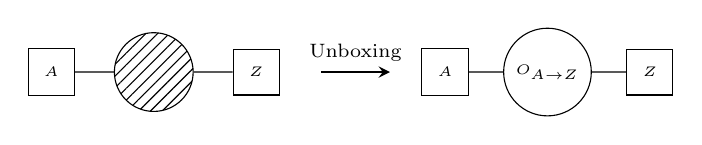
\begin{tikzpicture}[
    square/.style={regular polygon, regular polygon sides=4}
]
    % First diagram (left)
    \node at (0, 0) [circle, minimum size=1cm, draw, 
                    pattern={Lines[angle=45,distance=3pt]}] (cir1) {};
    \node at (-1.3, 0) [square, draw] (s1) {\tiny $A$};
    \node at (1.3, 0) [square, draw] (e1) {\tiny $Z$};
    \draw (s1.east) -- (cir1.west); 
    \draw (cir1.east) -- (e1.west);

    % Second diagram (right)
    \node at (5, 0) [circle, minimum size=0.8cm, draw] (cir2) {\tiny $O_{A \rightarrow Z}$};
    \node at (3.7, 0) [square, draw] (s2) {\tiny $A$};
    \node at (6.3, 0) [square, draw] (e2) {\tiny $Z$};
    \draw (s2.east) -- (cir2.west); 
    \draw (cir2.east) -- (e2.west);

    % Centered arrow between diagrams with "Unboxing" label
    \node at (2, 0) (midpoint) {};
    \draw[-stealth, thick] (midpoint) -- node[above] {\scriptsize Unboxing} ++(1,0);
\end{tikzpicture}
\end{document}
